\documentclass{article}
%\documentclass{minimal}
\usepackage[utf8]{inputenc}
\usepackage{relsize}
\usepackage{parskip}
\usepackage{amsmath}
\usepackage{amsfonts}
\usepackage{amssymb}
\usepackage{amsthm}
\usepackage{bbm}
\usepackage{mathtools}
\usepackage{bm} % bold symbols
\usepackage{multicol}
\usepackage{hyperref, framed}
\usepackage{pifont}
\usepackage{soul}
\hypersetup{
    colorlinks=true,
    urlcolor=blue,
    citecolor=black
}
\usepackage[nameinlink,noabbrev]{cleveref}
\usepackage{placeins}
\usepackage[margin=1in,footskip=0.5in]{geometry}
\usepackage{fancyhdr}
\usepackage{chngcntr}
\usepackage[shortlabels]{enumitem}
\usepackage{algorithm}
\usepackage{algpseudocode}
\newcommand{\crefrangeconjunction}{--}

\newcommand{\mat}[1]{\ensuremath{\bm{#1}}}
\newcommand{\cho}[2]{{#1 \choose #2}}
\newcommand{\cmark}{\ding{51}}
\newcommand{\dd}[2]{{\frac{\textrm{d}#1}{\textrm{d}#2}}}
\newcommand{\partiald}[2]{{\frac{\partial#1}{\partial#2}}}
\newcommand{\xmark}{\ding{55}}
\newcommand{\mybinom}[3][0.8]{\scalebox{#1}{$\dbinom{#2}{#3}$}}
\newcommand\numberthis{\addtocounter{equation}{1}\tag{\theequation}}
\DeclarePairedDelimiter\ceil{\lceil}{\rceil}
\DeclarePairedDelimiter\floor{\lfloor}{\rfloor}
\DeclarePairedDelimiter\abs{\lvert}{\rvert}
\DeclarePairedDelimiter\norm{\lVert}{\rVert}
% \newtheorem{lemma}{Lemma}
\DeclareMathOperator{\F}{\mathbb{F}}
\DeclareMathOperator{\N}{\mathbb{N}}
\DeclareMathOperator{\Z}{\mathbb{Z}}
\DeclareMathOperator{\Q}{\mathbb{Q}}
\DeclareMathOperator{\R}{\mathbb{R}}
\DeclareMathOperator{\C}{\mathbb{C}}
\DeclareMathOperator{\K}{\mathbb{K}}
\DeclareMathOperator{\B}{\textrm{B}}
\DeclareMathOperator{\E}{\mathbb{E}}
\DeclareMathOperator{\V}{\text{Var}}
\DeclareMathOperator{\dist}{\text{d}}
\DeclareMathOperator{\spn}{\text{span}}
\DeclareMathOperator{\im}{\text{Im}}
\DeclareMathOperator{\re}{\text{Re}}
\DeclareMathOperator{\col}{\text{col}}
\DeclareMathOperator{\sgn}{\text{sgn}}
\DeclareMathOperator{\X}{\mathcal{X}}
\newcommand{\rank}{\text{rank}}
\newcommand{\tr}{\text{tr}}
\DeclareMathOperator*{\argmax}{arg\,max\,}
\DeclareMathOperator*{\argmin}{arg\,min\,}
\DeclareMathOperator{\supp}{\text{supp}}

% \theoremstyle{definition}
\newtheorem{theorem}{Theorem}[section]
\newtheorem{corollary}{Corollary}[theorem]
\newtheorem*{proposition}{Prop}
\newtheorem{lemma}{Lemma} % \newtheorem{lemma}[theorem]{Lemma}
% \newtheorem{sublemma}{lemma}[lemma]
\newtheorem*{remark}{Remark}
\newtheorem*{fact}{Fact}
\newtheorem*{definition}{Def}
\newcounter{example}[section]
\newenvironment{example}[1][]{\refstepcounter{example}\par\medskip
   \textbf{Ex.~\theexample. #1} \rmfamily}{\medskip}
% \newtheorem{example}{Ex.}[section]

\title{QITE Write-up}
\author{Leon Lufkin}
\date{\today}

\makeatletter
\let\Title\@title
\let\Author\@author
\let\Date\@date
\makeatother

\pagestyle{fancy}
\lhead{\Title}
\chead{\Author}
\rhead{
\Date
}

\begin{document}
% \maketitle
% \allowdisplaybreaks

%%%%%%%%%%
%% QITE %%
%%%%%%%%%%
\section{QITE}
This implementation of quantum imaginary time evolution (QITE) is based on Motta (2020).
Imaginary time evolution (ITE), unlike ansatz-based approaches, always converges to the ground state.
The approach of Motta (2020) is unique in that it tries to approximate the ITE operator with a unitary operator, which can be implemented on a quantum computer.
In order to calculate this approximation, it requires one to perform $4^D$ measurements, where $D$ is the number of qubits, on a circuit with a number of gates scaling as $D 4^D N$, where $N$ is the number of timesteps in the simulation.

Given a $k$-local Hamiltonian $\hat{H} = \sum_{m} \hat{h}[m]$, the ITE operator is 
\begin{align}
    e^{-\beta \hat{H}} &= \left( e^{-\Delta \tau h[1]} \cdots e^{-\Delta \tau h[m]} \right)^{-\beta/\Delta \tau},
\end{align}
which acts on a state $\Psi$.
After a single Trotter step, we have
\begin{align}
    e^{-\Delta \tau \hat{h}[m]} | \Psi \rangle,
\end{align}
which we approximate as
\begin{align}
    e^{-i \Delta \tau \hat{A}[m]} | \Psi \rangle.
\end{align}
To compute $\hat{A}[m]$, we must first calculate the entries of the matrix $S$ and vector $b$ as
\begin{align} \label{eq:linear_eq}
    S_{J,J'} &= \langle \Psi | \hat{\sigma}_I^\dagger \hat{\sigma}_{I'} | \Psi \rangle, 
    \quad b_I = \frac{-i}{\sqrt{c}} \langle \Psi | \hat{\sigma}_I^\dagger \hat{h}[m] | \Psi \rangle,
\end{align}
where $J = j_1, \ldots, j_k$ is the index of $\sigma_J = \sigma_{j_1} \otimes \cdots \otimes \sigma_{j_k}$ and $c = \sqrt{ \langle \Psi | e^{-2 \Delta \tau \hat{h}[m]} | \Psi \rangle }$ is a normalization constant.
From this, one computes $a[m]$ by minimizing square-error in $S a[m] = b$.
Finally, we have $\hat{A}[m] = \sum_{J} a[m]_J \sigma_J$, which can be implemented on a quantum circuit.
Iteratively applying the $\hat{A}[m]$ yields the full ITE from $\Psi$ to the ground state.

%%%%%%%%%%%%%%%%%%%%
%% IMPLEMENTATION %%
%%%%%%%%%%%%%%%%%%%%
\section{Implementation}
The first part of our implementation of QITE is to decompose $\hat{H}$ in terms of the Pauli basis matrices $\hat{\sigma}_I, \hat{\sigma}_X, \hat{\sigma}_Y,$ and $\hat{\sigma}_Z$.
We do this using the Hilbert-Schmidt inner product.
Then, we compute all of the expectations in \cref{eq:linear_eq}.
Let $| \Psi \rangle$ be the state after evolving from $| 0 \rangle$ for $\beta$ units in imaginary time.
Then, we compute $e_J = \langle \Psi | \sigma_J | \Psi \rangle$ for all $J$.

Let us first define $\Sigma = \{(j_1,\ldots,j_k) : j_i \in \{I,X,Y,Z\} \}$.
Also define the map $(\cdot,\cdot) : \Sigma \times \Sigma \to \Sigma$ via $(J,J') = K$ s.t. $\sigma_J^\dagger \sigma_{J'} = c_K \sigma_K$, where $c_K \in \{\pm 1, \pm i\}$.
Recall the Pauli group $\{ \pm \sigma_I, \pm i \sigma_I, \pm \sigma_X, \pm i \sigma_X, \pm \sigma_Y, \pm i \sigma_Y, \pm \sigma_Z,$ $\pm i \sigma_Z \}$ is closed under multiplication ($\sigma_I$ is the identity operator).
Moreover, $\sigma_x^\dagger = \sigma_x$ holds for all $x \in \{I, X, Y, Z\}$.
Thus, there always exists an $l \in \{I,X,Y,Z\}$ s.t. $\sigma_j^\dagger \sigma_{j'} = \sigma_j \sigma_{j'} = c_l \sigma_l$.
For $J = j_1, \ldots, j_k$, observe that
\begin{align*}
    \sigma_J \sigma_{J'}
    &= (\sigma_{j_1} \otimes \cdots \otimes \sigma_{j_k}) (\sigma_{j'_1} \otimes \cdots \otimes \sigma_{j'_k})
    = (\sigma_{j_1} \sigma_{j'_1}) \otimes \cdots \otimes (\sigma_{j_k} \sigma_{j'_k}) \\
    &= (c_{l_1} \sigma_{l_1}) \otimes \cdots \otimes (c_{l_k} \sigma_{l_k})
    = \left( \prod_{i=1}^{k} c_{l_i} \right) \sigma_{l_1,\ldots,l_k}
    = c_L \sigma_L.
\end{align*}
Note that $\{\pm 1, \pm i\}$ is closed under multiplication, so $c_L \in \{\pm 1, \pm i\}$ as well.
Thus, $(\cdot,\cdot)$ exists and it is clearly well-defined.

Using the above function, we can easily find $S$ and $b$ as 
\begin{align}
    S_{J,J'}
    &= \langle \Psi | \sigma_I^\dagger \sigma_{I'} | \Psi \rangle
    = \langle \Psi | c_{(J,J')} \sigma_{(J,J')} | \Psi \rangle
    = c_{(J,J')} e_{(J,J')}.
\end{align}
Similarly, if we write $\hat{h}[m] = \sum_K c_K \sigma_K$, then
\begin{align}
    b_I &= \frac{-i}{\sqrt{c}} \langle \Psi | \hat{\sigma}_I^\dagger \hat{h}[m] | \Psi \rangle
    = \frac{-i}{\sqrt{c}} \sum_K c_K \langle \Psi | \hat{\sigma}_I^\dagger \sigma_K | \Psi \rangle
    = \frac{-i}{\sqrt{c}} \sum_K c_K c_{(I,K)} \langle \Psi | \hat{\sigma}_{(I,K)} | \Psi \rangle
    = \frac{-i}{\sqrt{c}} \sum_K c_K c_{(I,K)} e_{(I,K)}.
\end{align}
Therefore, we can compute $S$, $b$, and thus $a$ from the expectations $e_I$.
This allows us to perform one more ITE update.

In order to reduce the number of gates on the circuit (which scales as $D 4^D N$), I combined sequential gates of the same type.
For example, if a sequence of RX gates were applied to a qubit in a row, I would combine them into one gate.
Under this simplification, the number of gates is $(\sum_{d=1}^{D} 4^d) N = ((4^{D+1} - 1) / 3 - 1) N$, a reduction by about 30\% for $D=2$ and 67\% for $D=4$.

All quantum computation and simulation was performed using Qiskit.
I have typically been collecting $8,192$ shots for each quantum circuit.
I found that setting $\Delta \tau = 0.05$ was the largest timestep that achieved consistent results.
The code for this implementation can be found in my \href{https://github.com/leonlufkin/cognition_qite}{GitHub repo}.

%%%%%%%%%%%%%%
%% EXAMPLES %%
%%%%%%%%%%%%%%
\section{Examples}
\subsection{2 $\times$ 2 Hamiltonian from Motta (2020)}
$\hat{H} = \frac{1}{\sqrt{2}} \hat{\sigma}_X + \frac{1}{\sqrt{2}} \hat{\sigma}_Z$.
The true ground energy is $-1.0$.
\Cref{fig:2x2} shows that our QITE simulation matches that of Motta (2020) and correctly finds the ground energy of $\hat{H}$.
\begin{figure}
    \centering
    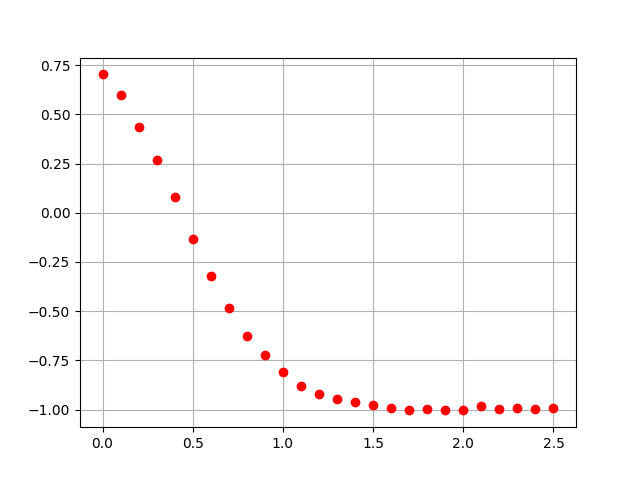
\includegraphics[width=0.4\textwidth]{2x2_Motta.png}
    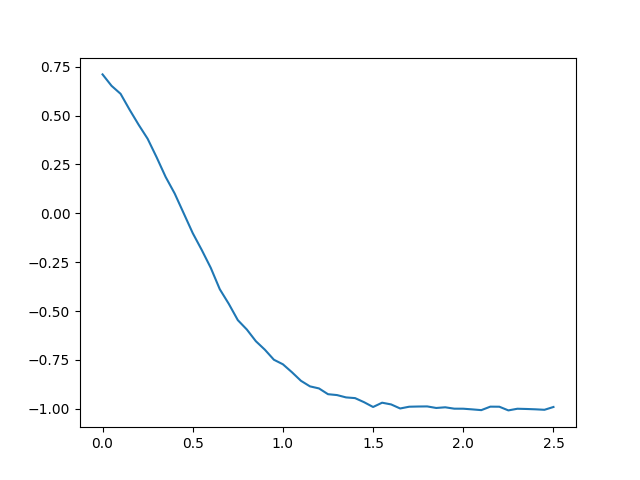
\includegraphics[width=0.4\textwidth]{2x2_ex.png}
    \caption{(Left) QITE simulation for $\hat{H}$ from Motta (2020) and (right) our QITE model.}
    \label{fig:2x2}
\end{figure}

\subsection{4 $\times$ 4 Hamiltonians}
$\hat{H}_1 = \hat{\sigma}_X \otimes \hat{\sigma}_Z + \hat{\sigma}_Y \otimes \hat{\sigma}_Z$ and $\hat{H}_2 = \hat{\sigma}_X \otimes \hat{\sigma}_Z$.
The true ground energy of $\hat{H}_1$ is $-1.414$ and that of $\hat{H}_2$ is $-1.0$.
\Cref{fig:4x4} shows that our simulation correctly finds the minimum ground energy for both Hamiltonians.
For $\hat{H}_1$, after finding the minmum energy, it evolves toward higher-energy states.
This issue is mentioned in \cref{sec:issues}.
\begin{figure}
    \centering
    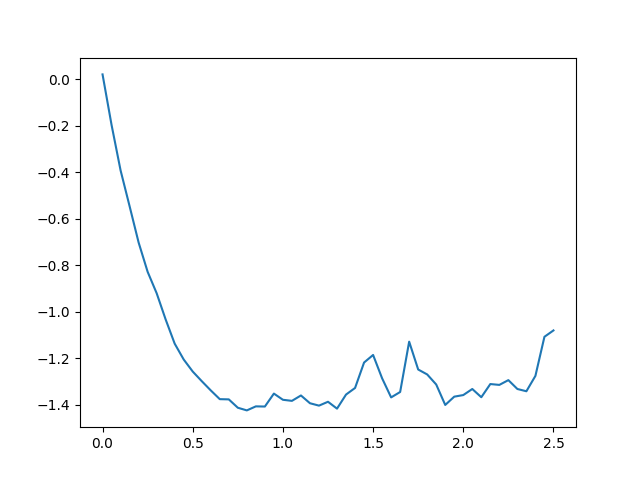
\includegraphics[width=0.4\textwidth]{4x4_ex1.png}
    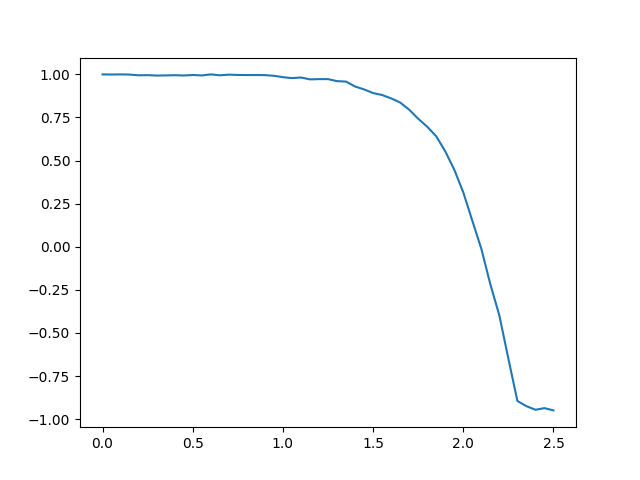
\includegraphics[width=0.4\textwidth]{4x4_ex2.png}
    \caption{Our model's QITE simulation for (left) $\hat{H}_1$ and (right) $\hat{H}_2$.}
    \label{fig:4x4}
\end{figure}

% \subsection{8 $\times$ 8 Hamiltonians}
% $\hat{H}_1 = \hat{\sigma}_X \otimes \hat{\sigma}_Z \otimes \hat{\sigma}_Y$.
% The true ground energy is $-1.0$.
% \Cref{fig:8x8} shows that our simulation correctly finds the minimum ground energy before evolving to higher-energy states.
% This issue is mentioned in \cref{sec:issues}.
% \begin{figure}
%     \centering
%     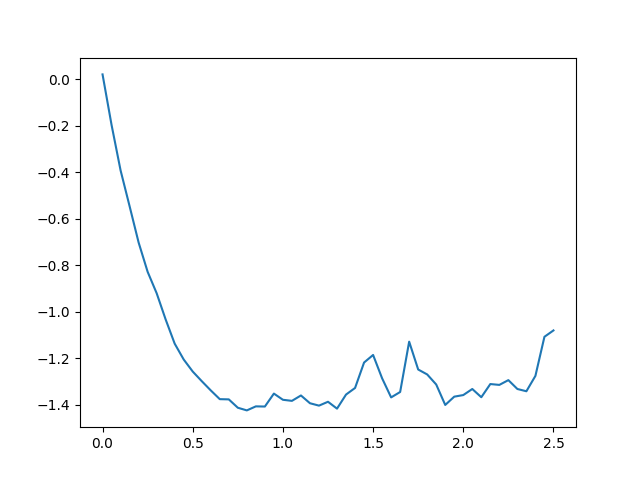
\includegraphics[width=0.4\textwidth]{4x4_ex1.png}
%     \caption{Our model's QITE simulation.}
%     \label{fig:8x8}
% \end{figure}


%%%%%%%%%%%%
%% ISSUES %%
%%%%%%%%%%%%
\section{Issues}
\label{sec:issues}
Our implementation of QITE suffers from several practical issues. % ; it is not clear if the implementation in Motta (2020) suffers from them as well.
First, the algorithm seems to struggle with larger Hamiltonians ($8 \times 8$ and larger).
That is, it does not decrease monotonically to the ground state energy.
Reducing $\Delta \tau$ appears to help with this issue, but it seems to depend on the complexity of the Hamiltonian (how many Pauli matrices appear in its linear decomposition).
I have not been able to find a rule for how to determine a suitable $\Delta \tau$ for arbitrary Hamiltonians.

Even when QITE does decrease monotonically to the ground state energy, it's behavior afterward is sometimes chaotic.
Take, for example, the left graph in \cref{fig:2x2}.
QITE correctly evolves the state toward the ground state for the first 1.0 imaginary seconds of the simulation.
However, after doing this, it appears to behave chaotically and evolves towards other states.
Motta (2020) discuss this issue, but the behavior they describe sounds less chaotic.

The QITE algorithm from Motta (2020) takes an extremely long time (at least one hour) to simulate on my machine for $8 \times 8$ Hamiltonians or larger.
This stems from exponential number of expectation calculations ($e_I$) required to calculate $\hat{A}[m]$.
This is the approach outlined in Motta (2020), and it does not appear to me that this can be subsstantially improved.
To me, requiring an exponential number of circuit measurement nullifies the quantum speedup provided by simulating the ground state.
This seems to be an inherent issue with the algorithm and encourages exploring other approaches.



\end{document}
